\documentclass{classrep}
\usepackage[utf8]{inputenc}
\frenchspacing

\usepackage{graphicx}
\usepackage{rotating}
\usepackage[usenames,dvipsnames]{color}
\usepackage[hidelinks]{hyperref}
\usepackage{float}
\usepackage[table,xcdraw]{xcolor}
\usepackage{amsmath, amssymb, mathtools}

\usepackage{fancyhdr, lastpage}
\pagestyle{fancyplain}
\fancyhf{}
\renewcommand{\headrulewidth}{0pt}
\cfoot{\thepage\ / \pageref*{LastPage}}

\renewcommand{\refname}{Bibliografia}

% bullet itemize
\renewcommand{\labelitemi}{\textbullet}

\studycycle{Informatyka stosowana, studia dzienne, II st.}
\coursesemester{II}

\coursename{Zastosowanie informatyki w medycynie}
\courseyear{2020/2021}

\courseteacher{dr hab. inż. Agnieszka Wosiak}
\coursegroup{środa, 13:30} %wpisałem start wykładu bo raz wykład raz laby

\author{%
\\
  \studentinfo[234053@edu.p.lodz.pl]{Paweł Galewicz}{234053}\\
  \studentinfo[234067@edu.p.lodz.pl]{Bartosz Jurczewski}{234067}\\
  \studentinfo[234102@edu.p.lodz.pl]{Zbigniew Nowacki}{234102}\\
  \studentinfo[234128@edu.p.lodz.pl]{Piotr Wardęcki}{234128}
}

\title{Zadanie 2: Niska waga urodzeniowa}

\begin{document}
\maketitle
\thispagestyle{fancyplain}
\clearpage

%%%%%%%%%%%%%%%%%%%%%%%%%%%%%%%%%%%%%%%%%%%%  Cel
\section{Cel}
Celem było zbadanie hipotezy: \textit{„Czy niska waga urodzeniowa naprawdę zmniejsza szanse na przeżycie dziecka powyżej jego pierwszych urodzin?”}.

%%%%%%%%%%%%%%%%%%%%%%%%%%%%%%%%%%%%%%%%%%%%  Opis implementacji
\section{Opis implementacji}
    Algorytmy oraz przygotowane do nich testy zostały zaimplementowane za pomocą języka Python w wersji 3.8.2.
    Wykorzystano w nim biblioteki \textit{NumPy}, \textit{Sklearn}, \textit{Pandas} i \textit{Seaborn}.

%%%%%%%%%%%%%%%%%%%%%%%%%%%%%%%%%%%%%%%%%%%%  Badania
\section{Badania}

    \subsection{Wpływ niedowagi na śmiertelność}
        \begin{table}[H]
            \centering
            \begin{tabular}{|l|c|}
                \hline
                \rowcolor[HTML]{FFCE93} 
                \multicolumn{1}{|c|}{\cellcolor[HTML]{FFCE93}\textbf{Kryterium}} & \textbf{Współczynnik} \\ \hline\hline
                Śmiertelność ciąży bliźniaczej z niedowagą                       & 3.80 \%               \\ \hline
                Śmiertelność ciąży bliźniaczej bez niedowagi                     & 0.53 \%               \\ \hline
                Całkowita śmiertelność ciąży bliźniaczej                         & 2.16 \%               \\ \hline\hline
                Śmiertelność u pojedynczej ciąży z niedowagą                     & 4.47 \%               \\ \hline
                Śmiertelność u pojedynczej ciąży bez niedowagi                   & 0.22 \%               \\ \hline
                Całkowity śmiertelność ciąży pojedynczej                         & 0.50 \%               \\ \hline
            \end{tabular}
        \end{table}
 
 %%%%%%%%%%%%%%%%%%%%%%%%%%%%%%%%%%%%%%%%%%%%      
    \subsubsection{Chi-kwadrat}
    
    Test chi-kwadrat używany jest między innymi do porównania ze sobą równoliczności kategorii dwóch rozkładów. Test wykorzystaliśmy do sprawdzenia równoliczności śmiertelności noworodków dla bliźniaków i jedynaków. Za hipotezę zerową przyjęliśmy, że liczebności są takie same:
    
    \begin{table}[H]
    \centering
    \caption{Błąd chi-kwadrat}
    \label{tab:error}
    \begin{tabular}{|l|l|}
    \hline
    \textbf{Chi-square statistic:} & 0.012977839125984913 \\ \hline
    \textbf{P-value:} & 0.9093009580356936 \\ \hline
    \end{tabular}
    \end{table}
    
    Na podstawie wartości parametru \textit{p} nie jesteśmy w stanie odrzucić hipotezy.
%%%%%%%%%%%%%%%%%%%%%%%%%%%%%%%%%%%%%%%%%%%%
    \subsection{Wpływ palenia u matki na wagę dziecka}
        \begin{figure}[H]
            \centering
            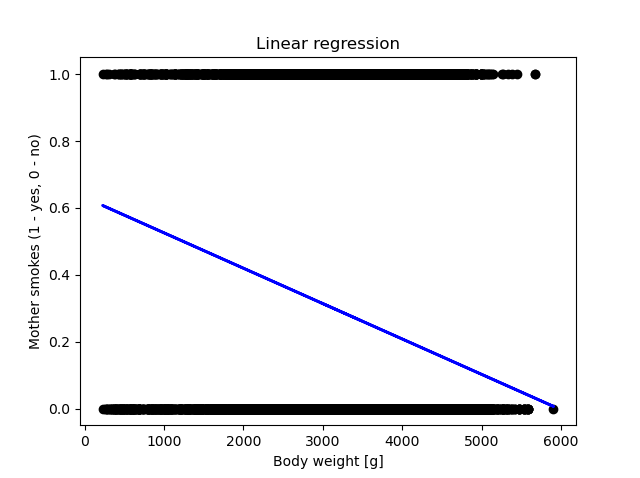
\includegraphics[width=0.9\textwidth]{images/images2/LinearRegression.png}
            \caption{Wpływ palenia u matki na masę urodzeniową dziecka}
            \label{fig1}
        \end{figure}
        
        \begin{figure}[H]
            \centering
            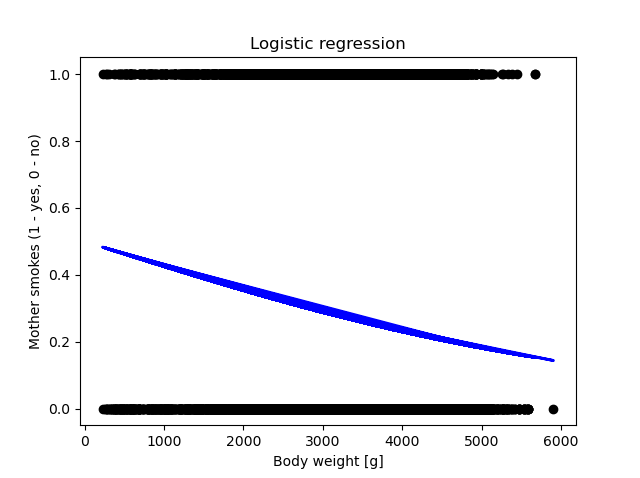
\includegraphics[width=0.9\textwidth]{images/images2/LogisticRegression.png}
            \caption{Wpływ palenia u matki na masę urodzeniową dziecka}
            \label{fig2}
        \end{figure}


%%%%%%%%%%%%%%%%%%%%%%%%%%%%%%%%%%%%%%%%%%%%
\section{Wnioski}

    \begin{itemize}
       
        \item Skupienie się na ciążach bliźniaczych wynika z chęci minimalizacji różnic środowiskowych już w trakcie życia bliźniąt.
        \item Powyższe badanie wskazuje, że palenie u matki ma wpływ na wagę urodzeniową dziecka. Dziecko rodzi się z mniejszą wagą.
        \item Niedowaga w ciąży bliźniaczej ma większy wpływ na śmiertelność niż w ciąży pojedynczej.
    \end{itemize}

\end{document}
